\section{Latent Spaces and Embeddings}
\label{sec:LatentSpacesAndEmbeddings}

In our work, we will often discuss the use of so-called \emph{embedding} for occlusion handling during the process of \gls{vot}. After an object emerges on a scene, there is an imminent need to assign it to either an existing track or mark the object as a new one. We believe the approach further described has the potential to significantly contribute to occlusion handling. To this end, one idea is to learn a metric embedding. 

% ########################################
\subsection{Learning Metric Embedding}
\label{ssec:LearningMetricEmbedding}

As~\cite{Hermans2017} describes, the goal of learning metric embedding is to learn a function (a transformation) $\func{f_\theta}{x}: \mathbb{R}^F \to \mathbb{R}^D$, which maps semantically similar points from the data manifold in $\mathbb{R}^F$ onto metrically close points in $\mathbb{R}^D$. Analogously, $\func{f_\theta}{\cdot}$ should map semantically different points in $\mathbb{R}^F$ onto metrically distant points in $\mathbb{R}^D$. Learning such a metric embedding is equivalent to dimensionality reduction, as it involves mapping a set of high dimensional input points onto a low dimensional manifold. The function $\func{f_\theta}{\cdot}$ ideally maps \emph{similar} (a measure of similarity has to be defined) points in the input space to nearby points on the manifold~\cite{Hadsell2006}.

To clarify, suppose the use of this transformation for vehicle \gls{reid}. This embedding would be achieved by a learned function that would map the images of vehicles into a latent space, where images of the same vehicle would be mapped closer together. Moreover, such a mapping should be invariant to variations in lighting conditions, vehicle rotations (a difficult one can be a change from front to rear view), and many other transformations that interfere with vehicle \gls{reid}.~\cite{Kuma2019} also mentions that popular loss functions for learning embeddings include contrastive or triplet loss, the two we will discuss further in the section \ref{ssec:SiameseAndTripletNetworks}. Among other things, embedding trained this way can be used to produce feature vector for classification, one-shot learning tasks~\cite{Koch2011}, clustering~\cite{Schroff2015}, face recognition~\cite{Parkhi2015} and last, but not least, re-identification~\cite{Kuma2019}.

Embedding, or mapping the input into some latent space with specific properties, is of great use even in combination with \glspl{gan}~\cite{Goodfellow2014}. A prominent work of researches from NVidia company~\cite{nvidia} demonstrates how individual facial features can be modified once the image of the person's face is mapped (embedded) into an adequate latent space~\cite{Karras2020}. Manipulations ranging from a change in hair and skin color through facial expressions (e.g. smile) up to the person's age or gender are possible using just linear vector operations. Briefly, once the user obtains the corresponding vector of the person's face image in the latent space formed during the training phase, then simply adding or subtracting a vector which corresponds to the \emph{age direction} results in making the person younger or older. All of this is achieved in a purely linear fashion. Even though such a generator architecture is by itself of no use for \gls{reid}, this approach initially led us to consider the exploration of latent spaces. Nonetheless, \glspl{gan} may provide a synthetically generated different views of the same vehicle (rear, front, etc.) to enhance the training on \emph{hard cases}~\cite{Lou2019} (further discussed in section \ref{ssec:TripletMiningStrategies}).

% ########################################
\subsection{Siamese and Triplet Networks}
\label{ssec:SiameseAndTripletNetworks}

\begin{figure}[t]
    \centering
    \begin{subfigure}[b]{0.49\textwidth}
        \centering
        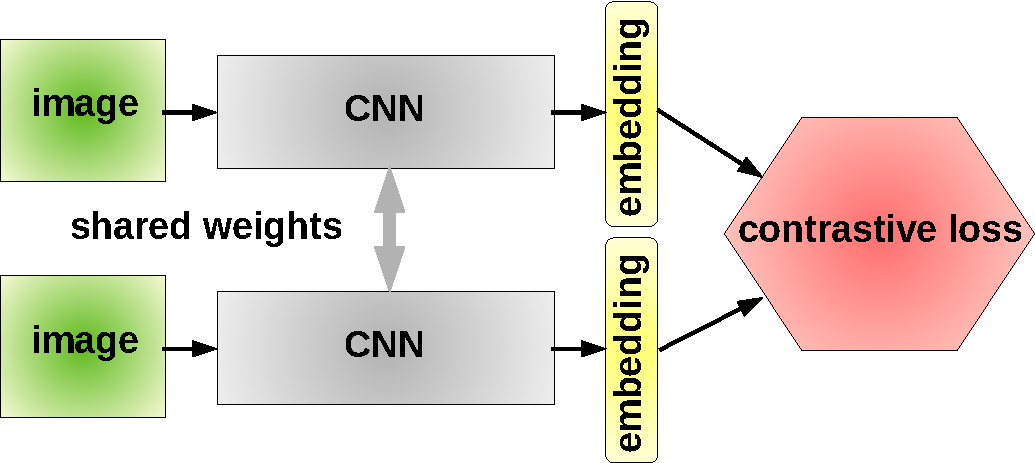
\includegraphics[width=\textwidth]{figures/theoretical_foundations/siamese_architecture.pdf}
        \caption[]{}
    \end{subfigure}
    \hfill
    \begin{subfigure}[b]{0.49\textwidth}
        \centering
        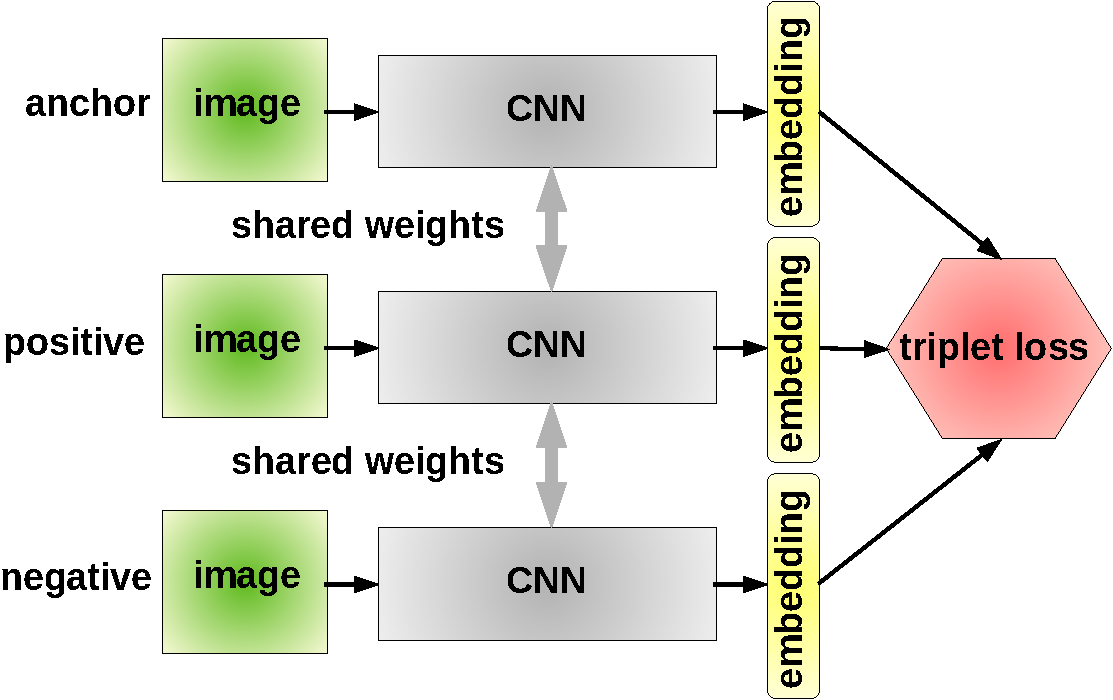
\includegraphics[width=\textwidth]{figures/theoretical_foundations/triplet_architecture.pdf}
        \caption[]{}
    \end{subfigure}
    \caption[Contrastive and triplet loss]{Comparison of the Siamese (a) and the triplet (b) network architectures. The concept of weight sharing implies that the same network is used for inference and only one set of weights is trained. Architectures are depicted as containing multiple models only for conceptual understanding.}
    \label{fig:SiameseAndTripletArchitectures}
\end{figure}

Let $\func{D}{x, y}: \mathbb{R}^D \times \mathbb{R}^D \to \mathbb{R}$ be a metric function measuring distances in the embedding space. Without a loss of generality, we will resort to use of the Euclidean distance ($L_2$ norm), so $\func{D}{x, y} = \euclnorm{x - y}$.

\subsubsection{Contrastive Loss}

Consider a sample $\rbrackets{x_0, x_1, y}$, where $x_0$ and $x_1$ represent the input, and the label $y = 1$ if $x_0$ and $x_1$ belong to the same category, otherwise $y = 0$. $\func{D}{\cdot}$ is the previously defined metric function, and $\alpha$ is the margin representing the minimum distance in the metric space to separate positive from negative samples. Then the contrastive function for any sample is defined as~\cite{Hadsell2006}

\begin{equation}
    \label{eq:ContrastiveLoss}
    \func{\mathcal{L}_{contr}}{\theta} = 
    \frac{1}{2}y
    {\func{D}{\func{f_\theta}{x_0}, \func{f_\theta}{x_1}}}^2 +
    \frac{1}{2}
    \rbrackets{1 - y} {\rbrackets{
    \sbrackets{\alpha - \func{D}{\func{f_\theta}{x_0}, \func{f_\theta}{x_1}}}_{+}}}^2.
\end{equation}

\noindent The two inputs $x_0$ and $x_1$ are fed to the shared model at the same time. The output is then evaluated by the contrastive loss function (Fig.~\ref{fig:SiameseAndTripletArchitectures} (a)). Positive samples should have a small distance between each other as measured by the $\func{D}{\cdot}$ to decrease the loss towards $0$. On the other hand, negative samples should have the distance beyond the threshold $\alpha$ to incur a loss of $0$.

\subsubsection{Triplet Loss}

\begin{figure}[t]
    \centerline{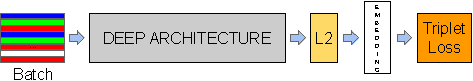
\includegraphics[width=0.8\linewidth]{figures/theoretical_foundations/triplet_loss_model_structure.pdf}}
    \caption[Triplet loss architecture]{A model structure developed by~\cite{Schroff2015}. This network consists of a batch input layer and a deep \gls{cnn} followed by an $L_2$ normalization, which produces the final embedding. A triplet loss is used during the training. \externalsrc{\cite{Schroff2015}}}
    \label{fig:TripletLossModelStructure}
\end{figure}

Apart from the contrastive loss, this time three samples are required to compute the loss. The rationale is to supply additional context when forming the metric space. Siamese networks are usually implemented using shared model weights, but there are better approaches when the triplet loss is used. Conceptually speaking, the model could be implemented as shown in Fig.~\ref{fig:SiameseAndTripletArchitectures} (b). However, as we will discuss later, triplet mining strategies are required for the triplet loss to work properly. The model can be thus simplified from an architectural point of view at the cost of moving the complexity to the computation of the loss function (see Fig.~\ref{fig:TripletLossModelStructure}).

Let $N$ be the number of all possible valid triplets $\rbrackets{x_a^i, x_p^i, x_n^i}$ for a given dataset. For any $i$-th triplet, let $x_a^i$ be the \emph{anchor} for a specific object (person, vehicle, etc.) with label $\func{y}{x_a^i}$, $x_p^i$ be the positive sample of the same object with label $\func{y}{x_p^i}$, such that $x_a^i \neq x_p^i \land \func{y}{x_a^i} = \func{y}{x_p^i}$, and let $x_n^i$ with label $\func{y}{x_n^i}$ be a sample of any other object, satisfying $\func{y}{x_a^i} \neq \func{y}{x_n^i}$, $\forall i = 1, \dots, N$. Let $\alpha$ be the margin value that is enforced between positive and negative pairs. Then, we want the relationship~\cite{Schroff2015}

\begin{equation}
    \label{eq:TripletDistanceConstraint}
    \func{D}{\func{f_\theta}{x_a^i}, \func{f_\theta}{x_p^i}} + \alpha < \func{D}{\func{f_\theta}{x_a^i}, \func{f_\theta}{x_n^i}}, \forall i = 1, \dots, N,
\end{equation}

\noindent to hold true. The triplet loss function is therefore defined as~\cite{Schroff2015}

\begin{equation}
    \label{eq:TripletLoss}
    \func{\mathcal{L}_{triplet}}{\theta} =
    \sum_{i = 1}^{N}
    {\sbrackets{
        \alpha +
        \func{D}{\func{f_\theta}{x_a^i}, \func{f_\theta}{x_p^i}} -
        \func{D}{\func{f_\theta}{x_a^i}, \func{f_\theta}{x_n^i}}
    }}_+.
\end{equation}

\noindent During the training with the triplet loss, the model should learn to push negative samples further away from the positive samples, ideally exceeding the margin $\alpha$. Assuming a situation when the negative sample is mapped closer than a positive sample, the training should result in the desired situation of bringing the positive sample closer while pushing the negative one further (see Fig.~\ref{fig:TripletLossLearningProcess}).

\begin{figure}[t]
    \centerline{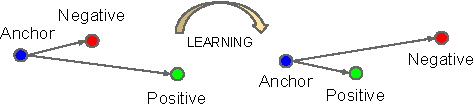
\includegraphics[width=0.7\linewidth]{figures/theoretical_foundations/triplet_loss_learning_process.pdf}}
    \caption[Triplet loss learning]{The objective is to learn embeddings such that the anchor is closer to the positive example than it is to the negative example by some margin value. The triplet loss, therefore, minimizes the distance between the anchor and the positive sample of the same identity and maximizes the distance between the anchor and the negative sample of a different identity. \externalsrc{\cite{Schroff2015}}}
    \label{fig:TripletLossLearningProcess}
\end{figure}

% ########################################
\subsection{Triplet Mining Strategies}
\label{ssec:TripletMiningStrategies}

Contrastive (eq. \ref{eq:ContrastiveLoss}) and triplet (eq. \ref{eq:TripletLoss}) loss functions play an important role in training an embedding model. However, the way that pairs or triplets are selected is crucial and as~\cite{Hermans2017} and~\cite{Manmatha2017} showed, it may significantly influence the training. They demonstrated that the sampling strategy matters at least as much as the loss function itself. Moreover, as the dataset gets larger, then the number of possible triplets grows cubically, rendering the use of all of them impractical. The majority of those triplets would be \emph{easy triplets}, thus hindering the learning process, because generating all possible triplets produces many triplets that fulfill the constraint \ref{eq:TripletDistanceConstraint}. To paraphrase the analogy from~\cite{Hermans2017}, showing the model that people with different clothes are not the same person after a certain point does not bring any new information. On the other hand, explicitly \emph{mining} images of similar-looking yet different people with the same clothes (\emph{hard negatives}) or of the same person with dramatically different poses (\emph{hard positives}) vastly contributes to an understanding of the notion of the \emph{same person}. As suggested, there are different kinds of triplets which are defined in the table \ref{tab:TripletCategoriesDefinitions}, using a general $\rbrackets{x_a^i, x_p^i, x_n^i}$ triplet for clarity. We encourage the reader to observe the figure \ref{fig:PositiveAndNegativeTripletsCategories}, too.

\begin{table}[t]
    \centering
    
    \begin{tabular}{|c|c|}
        \hline
        \tblcolname{triplet} & \tblcolname{constraint}\\
        \hline
        
        easy &
        $\func{D}{\func{f_\theta}{x_a^i}, \func{f_\theta}{x_p^i}} + \alpha < \func{D}{\func{f_\theta}{x_a^i}, \func{f_\theta}{x_n^i}}$\\
        \hline
        
        semi-hard&
        $\func{D}{\func{f_\theta}{x_a^i}, \func{f_\theta}{x_p^i}} < \func{D}{\func{f_\theta}{x_a^i}, \func{f_\theta}{x_n^i}} < \func{D}{\func{f_\theta}{x_a^i}, \func{f_\theta}{x_p^i}} + \alpha$\\
        \hline
        
        hard & $\func{D}{\func{f_\theta}{x_a^i}, \func{f_\theta}{x_n^i}} < \func{D}{\func{f_\theta}{x_a^i}, \func{f_\theta}{x_p^i}}$\\
        \hline
    \end{tabular}
    
    \caption{Definitions of various categories of triplets (regardless whether it is positive or negative) as imposed by their distance relationship.}
    \label{tab:TripletCategoriesDefinitions}
\end{table}

\begin{figure}[t]
    \centering
    \begin{subfigure}[b]{0.35\textwidth}
        \centering
        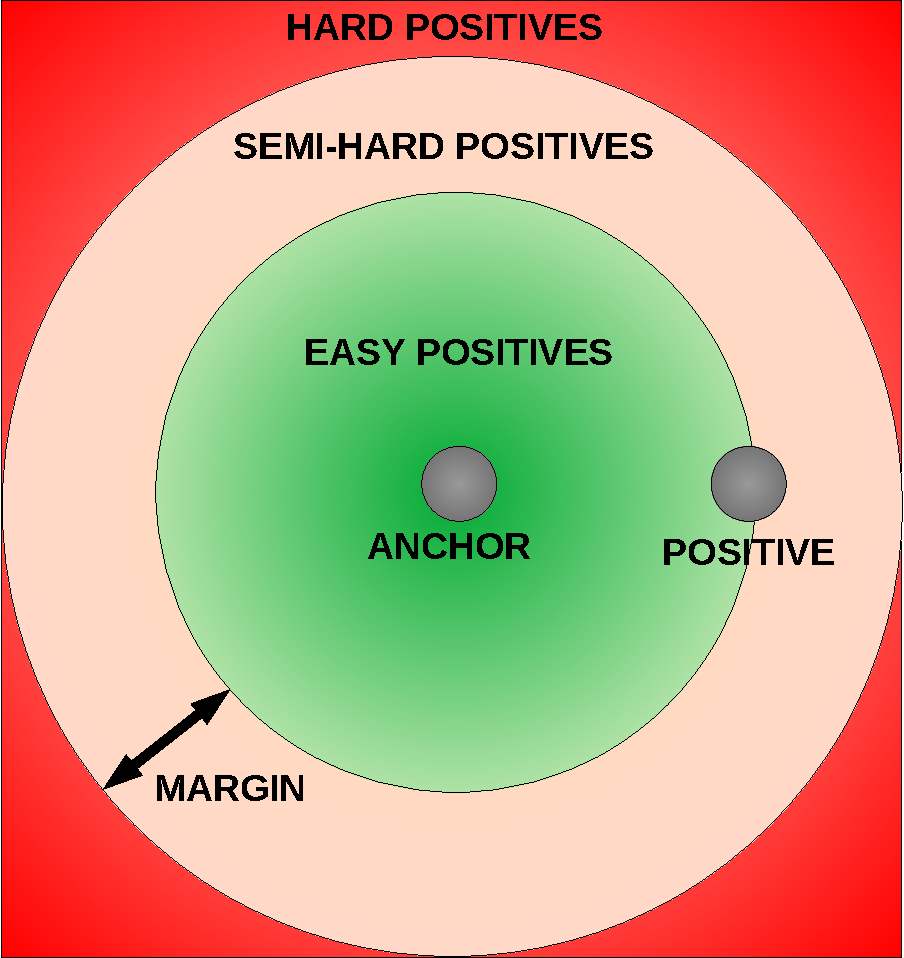
\includegraphics[width=\textwidth]{figures/theoretical_foundations/triplet_positives_categories.pdf}
        \caption[]{}
    \end{subfigure}
    \hfill
    \begin{subfigure}[b]{0.35\textwidth}
        \centering
        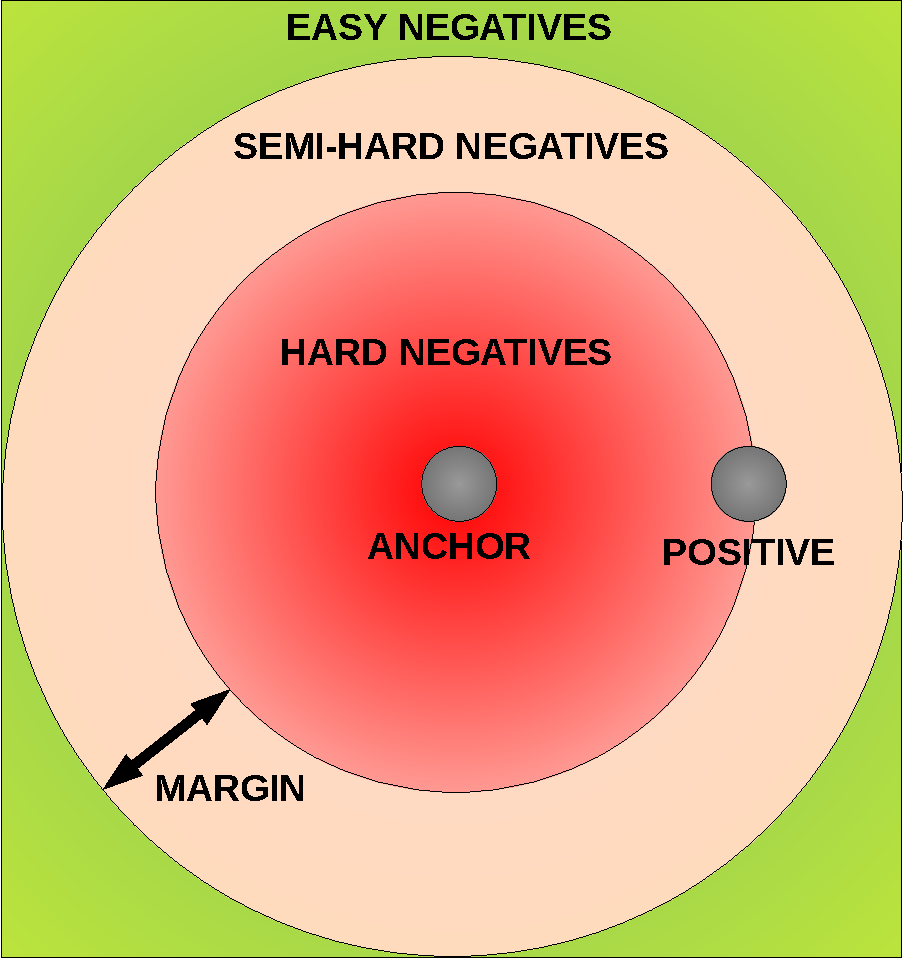
\includegraphics[width=\textwidth]{figures/theoretical_foundations/triplet_negatives_categories.pdf}
        \caption[]{}
    \end{subfigure}
    \caption[Triplet loss categories visualization]{Given a fixed anchor $x_a^i$ and positive sample $x_p^i$ as well as some positive margin value $\alpha$, we discriminate between three different types of categories in terms of their level of \emph{difficulty}. These categories vary in relation to positive (a) or negative (b) perspective.}
    \label{fig:PositiveAndNegativeTripletsCategories}
\end{figure}

In order to attain an effective convergence during the training, it is necessary to select triplets that violate the triplet constraint in the eq. \ref{eq:TripletDistanceConstraint}. This means that given $x_a^i$, the goal is to select a \emph{hard positive} $x_p^i$ given by $\argmax_{x_p^i}\cbrackets{\func{D}{\func{f_\theta}{x_a^i}, \func{f_\theta}{x_p^i}}}$ and a \emph{hard negative} $x_n^i$ as a result of $\argmin_{x_n^i}\cbrackets{\func{D}{\func{f_\theta}{x_a^i}, \func{f_\theta}{x_n^i}}}$. Admittedly, it is often infeasible to compute the $\argmin\cbrackets{\cdot}$ and $\argmax\cbrackets{\cdot}$ over the entire training set. In this regard, there are two possibilities to tackle this problem, either by selecting these hard triplets online or offline~\cite{Schroff2015}.

\subsubsection{Offline Triplet Mining}

Given a training set, the task is to produce reasonable triplets off-line, for instance, at the epoch beginning. First, a list of $N$ different valid triplets is randomly generated, then separated into $\lfloor \nicefrac{N}{B} \rfloor$ batches of $B$ triplets, followed by computation of $3N$ embeddings using the most recent network checkpoint. Each sample in a batch consists of a triplet, so the embedding has to be computed three times. Subsequently, hard or semi-hard triplets may be selected. Since this strategy has been shown on multiple occasions~\cite{Schroff2015, Hermans2017, Kuma2019} as an inferior choice compared to the on-line triplet mining, we will not discuss this approach further.

\subsubsection{Online Triplet Mining}

Online mining is performed by selecting the hard positive/negative exemplars from within a mini-batch (fig. \ref{fig:TripletArchitectureOnlineMining}). A condition that a minimum number of exemplars for any identity is present in each mini-batch has to be met. For example,~\cite{Schroff2015} used 40 different images of a single person (an identity) per mini-batch. Let $P$ be the number of different objects/identities (people, vehicles, etc.) and $K$ be the number of different images for a concrete identity (e.g. different views of the same vehicle). There are two prominent approaches to online mining: \emph{batch all} and \emph{batch hard}.

\begin{figure}[t]
    \centerline{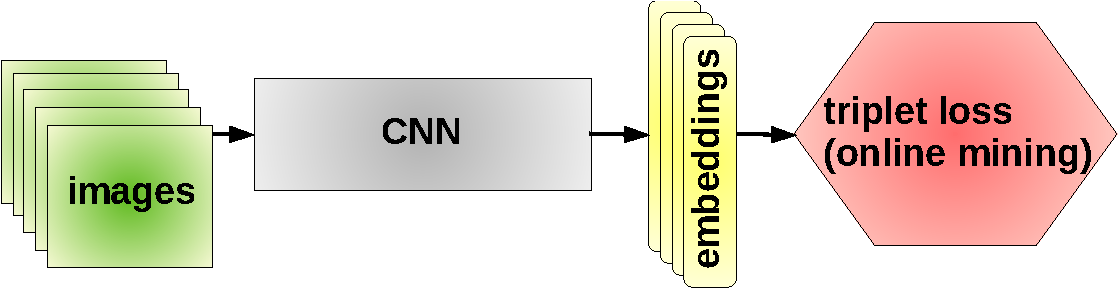
\includegraphics[width=0.55\linewidth]{figures/theoretical_foundations/triplet_architecture_online_mining.pdf}}
    \caption[Triplet loss online mining architecture]{The architecture of a triplet network where an online triplet loss function is used for training. In this architecture, no weight sharing is required as the triplet selection happens \emph{online} solely in the loss function.}
    \label{fig:TripletArchitectureOnlineMining}
\end{figure}

\subsubsection{Online Triplet Mining: Batch All}

This strategy aims for selecting all valid triplets and averaging the loss only on the hard and semi-hard triplets. Easy triplets (those for which the loss function equals $0$) are not taken into account as averaging on them would result in a very small loss, since they would usually vastly outnumber the set of harder triplets~\cite{Hermans2017}. This approach produces a total of $PK \rbrackets{K - 1} \rbrackets{PK - K}$ triplets ($PK$ anchors, $K - 1$ positives per anchors, $PK - K$ negatives) incorporated in the loss function as

\begin{equation}
    \label{eq:BatchAllLossFunction}
    \begin{aligned}
        \func{\mathcal{L}_{batchall}}{\theta} =
        \sum_{i = 1}^P
        \sum_{a = 1}^K
        \sum_{\substack{p = 1\\p \neq a}}^K
        \sum_{\substack{j = 1\\j \neq i}}^P
        \sum_{n = 1}^K
        \Bigg[
        &\alpha +\\
        &\func{D}{
            \func{f_\theta}{x_a^i},
            \func{f_\theta}{x_p^i}
        } -\\
        &\func{D}{
            \func{f_\theta}{x_a^i},
            \func{f_\theta}{x_n^j}
        }
        {\Bigg]}_{+}.
    \end{aligned}
\end{equation}

\subsubsection{Online Triplet Mining: Batch Hard}

In this strategy, the goal is to find the hardest positive and hardest negative for each anchor. The total number of triplets is $PK$. The selected triplets are the hardest among the given batch~\cite{Hermans2017}. Additionally,~\cite{Hermans2017} says that the selected triplets can be considered moderate, since they are the hardest within a small subset of the data, which is the best for learning with the triplet loss.

\begin{equation}
    \begin{aligned}
        \func{\mathcal{L}_{batchhard}}{\theta} =
        \sum_{i = 1}^P
        \sum_{a = 1}^K
        \Bigg[
            &\alpha +\\
            &\underset{p = 1, \dots, K} {\max}
            \cbrackets{
                \func{D}{
                    \func{f_\theta}{x_a^i},
                    \func{f_\theta}{x_p^i}
                }
            } -\\
            &\underset{\substack{j = 1, \dots, P\\n = 1, \dots, K\\j \neq i}} {\min}
            \cbrackets{
                \func{D}{
                    \func{f_\theta}{x_a^i},
                    \func{f_\theta}{x_n^j}
                }
            }
        {\Bigg]}_{+}
    \end{aligned}
\end{equation}

% ########################################
\subsection{Training Embeddings Using Adversarial Learning}
\label{ssec:TrainingEmbeddingsAdversarialLearning}

As we have seen so far, the mining of \emph{hard} samples (pairs or triplets) is crucial for training the embedding model. Nevertheless, as the model improves, it is essential to provide \emph{harder} samples every time. It can be observed in the contrastive (equation~\ref{eq:ContrastiveLoss}) or the triplet loss (equation~\ref{eq:TripletLoss}) functions, that once the negative sample is \emph{pushed} beyond the margin boundary, this sample incurs a $0$ contribution to the loss. It, therefore, is appropriate to constantly provide \emph{harder} samples as the model progresses, but the number of hard samples within the training set naturally decreases. One way to achieve this is to utilize adversarial training, the concept introduced by~\cite{Goodfellow2014}. An architecture called the Embedding Adversarial Learning Network, proposed by~\cite{Lou2019} is capable of generating synthetic samples in the embedding space. The advantage of harnessing this scheme is that instead of mining abundant \emph{hard} samples from the training set, which may be remarkably laborious, if not impossible, the automatically generated \emph{hard} samples can greatly improve the network's capability for discriminating similar objects~\cite{Lou2019}. Since~\cite{Lou2019} also deal with the problem of vehicle \gls{reid}, their approach improves the robustness of the embedding model to queries with different views of vehicles, because they employ \emph{hard negative} mining and \emph{cross-view} generation during the training. Identification of the corresponding rear viewpoint of a vehicle given only its front viewpoint and vice versa casts a challenge for the \gls{reid} methods.

Their contribution encompasses a novel adversarial scheme based on feature distance within the embedding space. Following the notation from~\cite{Lou2019}, let $x$ be an input sample, and $\func{G}{x}$ be a generated sample using the generator $G$. $\func{G}{x}$ is constrained to be close to the given sample $x$, within a relative positive margin $\alpha$, in the target embedding space. On the contrary, let $D_{emb}$ be the discriminator the purpose of which is to push the $\func{G}{x}$ away from $x$ while aiming to make the relative distance to be greater than $\alpha$. Simply put, the generator $G$ attempts to minimize the feature distance while the discriminator $D_{emb}$ tries to maximize it (Fig.~\ref{fig:EALNDiscriminatorGeneratorScheme}). This adversarial scheme can be formulated as follows,

\begin{equation}
    \begin{aligned}
        &\underset{G}{\min} \ \underset{D_{emb}}{\max} \ \mathbb{E}_{x \sim \func{pdata}{x}} \max \cbrackets{\func{d}{x, \func{G}{x}} - \alpha, 0},\\
        &\func{d}{x, \func{G}{x}} = \euclnorm{\func{D_{emb}}{x} - \func{D_{emb}}{\func{G}{x}}}^2,
    \end{aligned}
\end{equation}

\noindent with $\func{D_{emb}}{x}$ being the mapping of $x$ to the embedding space through the discriminator $D_{emb}$~\cite{Lou2019}. As~\cite{Goodfellow2014} proposed in his initiative work on \glspl{gan}, the generator and the discriminator are trained alternatively in this scheme as well.

\begin{figure}[t]
    \centerline{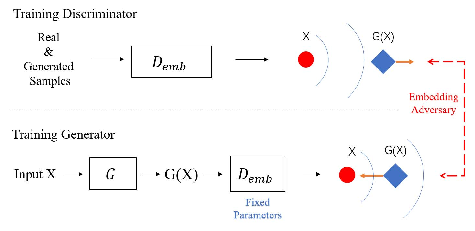
\includegraphics[width=0.8\linewidth]{figures/theoretical_foundations/ealn_discriminator_generator_scheme.pdf}}
    \caption[Embedding adversarial learning architecture]{Adversarial learning between the generator $G$ and the discriminator $D_{emb}$. The generator $G$ tries to produce samples close to the given sample $x$ in the embedding space, while the discriminator $D_{emb}$ tries to push those samples far away from each other, beyond the margin $\alpha$~\cite{Lou2019}.}
    \label{fig:EALNDiscriminatorGeneratorScheme}
\end{figure}

Their approach encompasses multiple stages. The first one is the \emph{embedding adversarial learning}, the design principle of which is manipulating the generation of the samples in the embedding space. Later on, the aforementioned first stage is extended by the \emph{hard negative adversarial learning}, which consists of two parts, i.e., the \emph{embedding adversarial learning} and the \emph{real-fake adversarial learning}. Another concurrent stage is introduced, called the \emph{cross-view adversarial learning}. Based on the \emph{embedding adversarial learning}, the aim is to address the issue of vehicle feature match-ing between different views via cross-view generation.
